\documentclass[12pt]{bsc}

\usepackage[T1,MeX]{polski}
\usepackage[utf8]{inputenc}
\usepackage[T1]{fontenc}
\usepackage{txfonts}

\usepackage{graphicx}
\usepackage{fancyvrb}
\usepackage{pdfpages}

\usepackage{enumitem}
\usepackage{listings}
\usepackage{caption}

\usepackage{alltt}

%sposob na zablokowanie obrazka na stronie
%\FloatBarrier (wcześniej dołącz \usepackage{placeins})
\usepackage{placeins}


%caption listingów
\DeclareCaptionFont{black}{ \color{black} }
\DeclareCaptionFormat{listing}{
  {
    \parbox{\textwidth}{\hspace{12pt}#1#2#3}
  }
}
\captionsetup[lstlisting]{ format=listing, labelfont=black, textfont=black, singlelinecheck=false, margin=0pt, font={bf,footnotesize} }

%definicja custom listingów
\lstdefinestyle{custom}{
  breaklines=true,
  xleftmargin=\parindent,
  showstringspaces=false,
  basicstyle=\fontsize{10}{11}\selectfont,
}

%pozwala na używanie znaku dolara($) w listingach
\lstset{
    mathescape=false
}

\usepackage[pdftex,pdfstartview=FitH,unicode]{hyperref}
% "klikalny" spis treści
\hypersetup{
    colorlinks,
    citecolor=black,
    filecolor=black,
    linkcolor=black,
    urlcolor=black
}

%https://tex.stackexchange.com/questions/36880/insert-a-blank-page-after-current-page
\usepackage{afterpage}

\newcommand\blankpage{%
    \null
    \thispagestyle{empty}%
    \addtocounter{page}{-1}%
    \newpage}
    


\graphicspath{{./img/}}

\selecthyphenation{polish}


% ********* documents meta data **********
\makeatletter

\def\@title{Tytuł pracy inżynierskiej}
\def\@engTitle{English title of your engineers work}
\def\@author{Jan Kowalski}
\def\@promoter{Dr inż. Alfred Kowalski}
\def\@when{2019-01-28}
\def\@year{2019}
\def\@album{9999}

\makeatother

\renewcommand{\partname}{}

\begin{document}
  \thispagestyle{empty}

\makeatletter

\begin{titlepage}
  \sffamily\bfseries
  
  \center{
    \fontsize{18}{18}\selectfont{
      WYŻSZA SZKOŁA INFORMATYKI I ZARZĄDZANIA
      ,,COPERNICUS'' WE WROCŁAWIU
    }
    \rule[10pt]{\textwidth}{1pt}
    \raisebox{12pt}[0px]{
      \fontsize{16}{16}\selectfont{WYDZIAŁ INFORMATYKI, ADMINISTRACJI I FIZJOTERAPII}
    }
  }
  
  \flushleft\fontsize{14}{14}\selectfont{
    \parbox{110pt}{\textmd{Kierunek studiów:}}
    Informatyka

    \parbox{110pt}{\textmd{Poziom studiów:}}
    Studia pierwszego stopnia-inżynierskie
    
    \parbox{110pt}{\textmd{Specjalność:}}
    Systemy i sieci komputerowe
  }
  
  \vspace*{40pt}
  \center{
    \fontsize{14}{14}\selectfont{PRACA DYPLOMOWA INŻYNIERSKA}
    
    \vspace*{30pt}
    \fontsize{14}{14}\selectfont\@author
    
    \vspace*{15pt}
    \fontsize{20}{20}\selectfont\@title
    
    \vspace*{20pt}
    \fontsize{14}{14}\selectfont\@engTitle
  }

  \vspace*{80pt}
  \flushright{  
    \fontsize{14}{14}\selectfont{Ocena pracy:}
    \makebox[220pt][r]{\fontsize{10}{10}\selectfont\dotfill}
    
    \fontsize{10}{10}\selectfont\textmd{(ocena pracy dyplomowej, data, podpis promotora) }
    
    \vspace*{50pt}
    \makebox[220pt][r]{\fontsize{10}{10}\selectfont\dotfill}
    
    \raisebox{4pt}{\fontsize{10}{10}\selectfont\textmd{(pieczątka uczelni)}}
  }
    
  \flushleft\fontsize{14}{14}\selectfont{
    Promotor:
    
    \bigskip\@promoter
  }

  \vspace*{20pt}
  \center{
    \rule[3pt]{\textwidth}{1pt}
    \fontsize{16}{16}\selectfont{WROCŁAW \@year}
  }
\end{titlepage}

\makeatother

\clearpage


  \tableofcontents
  
  \chapter{Wstęp}

\section{Wprowadzenie}

\section{Cel pracy}

\section{Motywacja}

\section{Zakres}

  
  \part{Część przeglądowa}  
  \chapter{Część przeglądowa}

\section{Przykładowa sekcja}


\subsection{Przykładowa subsekcja}
Quia ipsam non animi placeat amet sed. Cumque aut ratione velit expedita occaecati rerum qui. Cumque aut et quo repellat. Dolorem minima molestiae accusamus laboriosam qui. Neque quam qui natus optio quae. Przykładowy Refferal do obrazka nr \ref{fig:przykladowy-obrazek}.

\begin{figure}[ht]
        \centering
        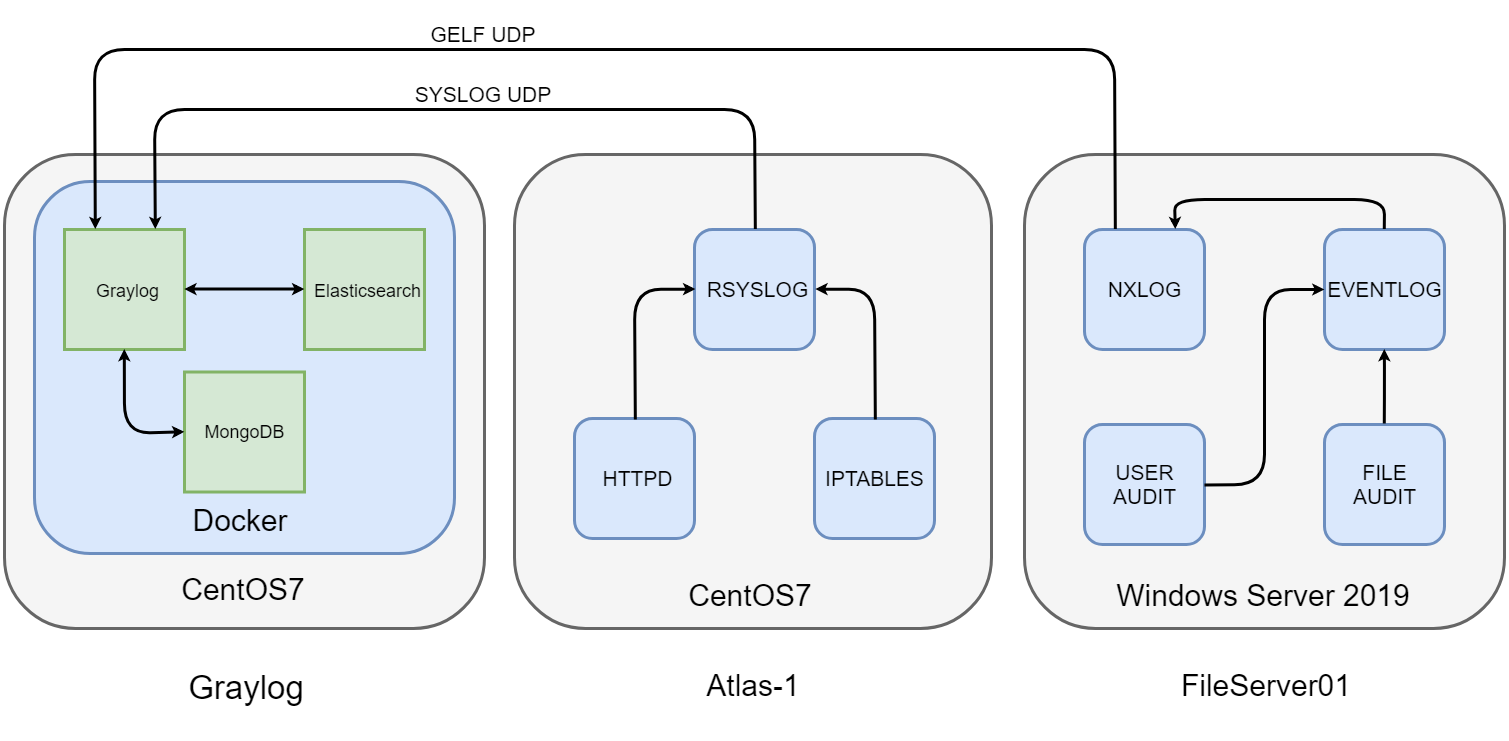
\includegraphics[width=16cm]{przykladowy-obrazek.png}
        \caption{Podpis obrazka i odnośnik do bibliografii \cite{przykladowy-obrazek}}
        \label{fig:przykladowy-obrazek}
\end{figure}

\newpage

\section{Druga sekcja}
Quia ipsam non animi placeat amet sed. Cumque aut ratione velit expedita occaecati rerum qui. Cumque aut et quo repellat. Dolorem minima molestiae accusamus laboriosam qui. Neque quam qui natus optio quae. Przykładowy Refferal do obrazka nr \ref{table:przykladowa-tabela}.

\begin{table}[htb]
	\centering
	\caption{Przykładowa tabela}
	\label{table:przykladowa-tabela}

    \begin{tabular}{| l | l |}
    \hline
    Nazwa komponentu & Licencja \\ \hline
    Graylog 2.5 & GNU General Public License v3 \\ \hline
    MongoDB 3.4 & GNU Affero General Public License v3 \\ \hline
    Elasticsearch 6.5.1 & Elastic License \cite{elastic-license} \\ \hline
    rsyslog 8.24.0 & GNU General Public License v3  \\ \hline
    NXLog CE 2.10.2150& NXLog Public License  \\ \hline
    Docker 18.09.1 & Apache License 2.0  \\
    \hline
    \end{tabular}
\end{table}

\newpage


  \part{Część praktyczna}
  \chapter{Część praktyczna}

\section{}

\subsection{}

Do listingów też można zrobić odniesienie np poniżej mamy listing nr \ref{listing:przykladowy}

%zmiana nazwy listingów
\renewcommand{\lstlistingname}{Listing}

\begin{lstlisting}[caption=Przykładowy listing pliku konfiguracyjnego , label=listing:przykladowy]
<Extension _syslog>
 Module xm_gelf
</Extension>

<Input in>
 Module	im_msvistalog
</Input>

<Output out>
 Module      om_udp
 Host        192.168.21.211
 Port        12201
 OutputType  GELF
</Output>

<Route 1>
 Path        in => out
</Route>
\end{lstlisting}

%czyści puste strony
\let\cleardoublepage\clearpage
  
  \chapter{Podsumowanie}


%czyści puste strony
\let\cleardoublepage\clearpage

  \pagestyle{plain}
  \cleardoublepage
\phantomsection
\addcontentsline{toc}{chapter}{Bibliografia}


\begin{thebibliography}{99}
%Literatura:

  \bibitem{przykladowy-obrazek}
  G. Skornowicz,
  \emph{Twórczość własna},
  wyd V, wyd. Helion, 
  Wrocław 2019
  
%przykladowy wpis:
  \bibitem{linux-security}
  M. Rash,
  \emph{Bezpieczeństwo sieci w linuksie},
  Wyd I, wyd. Helion,
  Gliwice 2008
  
%przykladowy wpis:
 \bibitem{linux-server}
	C. Binnie
	\emph{Linux Server: Bezpieczeństwo i ochrona sieci},
	Wyd I, wyd. Helion,
	Gliwice 2017
	
\end{thebibliography}


% Opis bibliograficzny wydawnictwa zwartego (książki) składa się z następujących pozycji [7]:
% autorzy (nazwisko + inicjały imion), tytuł (kursywa bez cudzysłowu), nazwa wydawnictwa,
% miejsce wydania, rok wydania (w nawiasach). Poszczególne części opisu powinny być
% oddzielone przecinkami. Przy dużej liczbie autorów można podać dane pierwszego autora z frazą
% „et al.” [5].
% 
% Opis artykułu w czasopiśmie [2,9]: autorzy (nazwisko + inicjały imion), tytuł (kursywa bez
% cudzysłowu), nazwa czasopisma, wolumin, numer, rok wydania (w nawiasach), strony „od–do”
% przedzielone znakiem półpauzy (Alt+0150), bez spacji w środku.
% 
% Opis referatu w materiałach konferencyjnych lub rozdziału pracy zbiorowej [4]: autorzy
% referatu (nazwisko + inicjały imion), tytuł referatu (kursywa bez cudzysłowu), słowo (w:),
% redaktorzy pracy zbiorowej (nazwisko + inicjały imion), słowo (red.), tytuł pracy zbiorowej lub
% dane konferencji (czcionka prosta), wydawnictwo, miejsce wydania, rok wydania (w nawiasach),
% strony „od–do” przedzielone znakiem półpauzy (Alt+0150), bez spacji w środku. Jeżeli
% opisywana praca jest częścią serii wydawniczej, należy dodać jej nazwę oraz numer woluminu
% pomiędzy tytułem pracy zbiorowej i nazwą wydawnictwa [6]. Możliwe jest także zastosowanie
% skróconego opisu referatu w materiałach konferencyjnych – bez podawania redaktorów i tytułu
% pracy zbiorowej [1].
% 
% W opisie materiałów publikowanych elektronicznie (np. specyfikacji, dokumentacji
% technicznej) należy umieścić dane autora lub nazwę producenta (jeśli nie ma podanego autora),
% tytuł dokumentu, ewentualnie opis rodzaju dokumentu (np. podręcznik użytkownika), wydawcę
% i rok wydania (w nawiasach) [8]. Opis strony internetowej składa się z danych autora albo nazwy
% organizacji publikującej, tytułu dokumentu albo nazwy serwisu, jego adresu URL (bez
% podkreślenia i niebieskiego koloru), roku opublikowania oraz daty odczytania dokumentu4 [3].
% 
% 1. Agrawal R., Srikant R., Fast Algorithms for Mining Association Rules, Proceedings
% of the Twentieth International Conference on Very Large Databases, Santiago, Chile
% (1994)
% 2. Bacchus F., Grove A., Halpern J., Koller D., From statistical knowledge bases
% to degrees of belief, Artificial Intelligence, Vol. 87, No. 1–2 (1996) 75–143
% 3. Brown D., A Beginners Guide to UML. Part 1–2., Dunstan Thomas Consulting,
% http://consulting.dthomas.co.uk (2002), (odczytano 10 września 2008 r.)
% 4. Deogun J., Jiang L., Comparative Evaluation on Concept Approximation Approaches,
% (w:) Kwaśnicka H., Paprzycki M. (red.), Proceedings of the Fifth International
% Conference on Intelligent Systems Design and Applications, IEEE Computer Society
% Press, Washington, Brussels, Tokyo (2005) 438–443
% 5. Fagin R. et al., Reasoning About Knowledge, MIT Press, Cambridge, USA (1995)
% 6. Kazakov D., Kudenko D., Machine Learning and Inductive Logic Programming for
% Multi-Agent Systems, (w:) Luck M., Marik V., Stepankova O. (red.), Multi-Agent
% Systems and Applications, Lecture Notes in Artificial Intelligence (LNAI), Vol. 2086,
% Springer-Verlag, Berlin Heidelberg (2001) 246–270
% 7. Kerninghan B.W., Ritchie D.M., Język ANSI–C, Wydawnictwa Naukowo-Techniczne,
% Warszawa (1994)
% 8. Microsoft, Books On-Line, dokumentacja elektroniczna systemu MS SQL Server 2000
% Enterprise Edition, Microsoft Corporation (2000)
% 9. Perry P., Walnum C., Pierwsze kroki Telefonii GSM, Kwartalnik Elektroniki
% i Telekomunikacji, Vol. 43, No. 3 (1997) 421–430

  
  \cleardoublepage
\phantomsection
\addcontentsline{toc}{chapter}{Spis rysunków}
\listoffigures

\cleardoublepage
\phantomsection
\addcontentsline{toc}{chapter}{Spis tabel}
\listoftables

\cleardoublepage
\phantomsection
\addcontentsline{toc}{chapter}{Spis listingów}
\renewcommand{\lstlistlistingname}{Spis listingów}
\lstlistoflistings

%czyści puste strony
\let\cleardoublepage\clearpage

  \cleardoublepage
\newgeometry{tmargin=3.3cm,bmargin=2.0cm,lmargin=2.0cm,rmargin=2.0cm,bindingoffset=1.0cm,nomarginpar,nohead}
\thispagestyle{plain}

\phantomsection
\addcontentsline{toc}{chapter}{Zawartość płyty CD}

Zawartość płyty CD
\begin{enumerate}
\item praca.pdf;
\item Plik z kodem źródłowym: xxx.js;
\item Plik z kodem źródłowym: yyy.css;
\item Plik z kodem źródłowym: zzz.html;
\end{enumerate}

  
  \addcontentsline{toc}{chapter}{Załączniki}

\addcontentsline{toc}{section}{Załącznik 1}
Załącznik 1 - zawartość skryptu przykladowy\_skrypt.sh
\lstinputlisting[style=custom,nolol]{./src/przykladowy_skrypt.sh}

\newpage
  
  % załącznik nr 5
% Made by Mateusz Cedro

\addcontentsline{toc}{chapter}{Oświadczenie o udostępnianiu pracy dyplomowej} % dodanie do spisu treści

\makeatletter
\newgeometry{tmargin=3.3cm,bmargin=2.0cm,lmargin=2.0cm,rmargin=2.0cm,bindingoffset=1.0cm,nomarginpar,nohead}

\begin{flushright}
    Wrocław, dnia \@when
  \end{flushright}

  \begin{flushleft}
    {\fontsize{14}{14} \selectfont
    
    \vspace*{20pt}
    {\bf Wydział Informatyki, Administracji i Fizjoterapii}
    
    \bigskip
    Kierunek studiów: {\bf informatyka (INF)}
    }  
  \vspace*{30pt}
  
  {~\@author} % autor pracy
  \vspace*{-4pt}
  
  \makebox[220pt][r]{\dotfill} %zastępuję dotline

  \vspace*{-2pt}
  {\scriptsize (imię i nazwisko studenta)}

  \bigskip
  {~\@album} %nr indeksu
  
  \vspace*{-4pt}
  \makebox[220pt][r]{\dotfill} %zastępuję dotline
  
  \vspace*{-2pt}
  {\scriptsize (nr albumu)}
\end{flushleft}

  \bigskip

\begin{center}
  {\fontsize{16}{16} \selectfont \bf OŚWIADCZENIE O UDOSTĘPNIANIU PRACY DYPLOMOWEJ}
\end{center}

\bigskip

\begin{flushright} %parbox potrafi dzielić linie. Mbox - nie.
    \vspace*{-4pt}
    \parbox{350pt}{
        Tytuł pracy dyplomowej: ~\@title
      }
\end{flushright}

\bigskip

\begin{flushright}
  Wyrażam zgodę (nie wyrażam zgody)\footnote{Niepotrzebne skreślić.} na udostępnianie mojej pracy dyplomowej.
\end{flushright}

\bigskip

\vspace*{30pt}
\begin{flushright} % wyrownanie do prawej
    \makebox[150pt]{\dotfill} % wypełniamy kropkami box
  
  \vspace*{-2pt}
  \makebox[150pt]{\scriptsize (podpis studenta)} % nowy box z podpisem
\end{flushright}

\restoregeometry
\makeatother
  
  % załącznik nr 6
% Made by Mateusz Cedro
\addcontentsline{toc}{chapter}{Oświadczenie autorskie} % dodatkowy wpis do spisu treści

\makeatletter
\newgeometry{tmargin=3.3cm,bmargin=2.0cm,lmargin=2.0cm,rmargin=2.0cm,bindingoffset=1.0cm,nomarginpar,nohead}

\begin{flushright}
    Wrocław, dnia \@when
  \end{flushright}

  \begin{flushleft}
    {\fontsize{14}{14} \selectfont
    
    \vspace*{20pt}
    {\bf Wydział Informatyki, Administracji i Fizjoterapii}
    
    \bigskip
    Kierunek studiów: {\bf informatyka (INF)}
    }  
  \vspace*{30pt}
  
  {~\@author} % autor pracy
  \vspace*{-4pt}
  
  \makebox[220pt][r]{\dotfill} %zastępuję dotline

  \vspace*{-2pt}
  {\scriptsize (imię i nazwisko studenta)}

  \bigskip
  {~\@album} %nr indeksu
  
  \vspace*{-4pt}
  \makebox[220pt][r]{\dotfill} %zastępuję dotline
  
  \vspace*{-2pt}
  {\scriptsize (nr albumu)}
\end{flushleft}

  \bigskip

\begin{center}
  {\fontsize{16}{16} \selectfont \bf OŚWIADCZENIE AUTORSKIE}
\end{center}

\bigskip


    Oświadczam, że niniejszą pracę dyplomową pod tytułem:
    \begin{center}
        {\fontsize{16}{16} \selectfont \bf \@title}
    \end{center}
    napisałem/am samodzielnie. Nie korzystałem/am z pomocy osób trzecich, jak również nie dokonałem/am zapożyczeń z innych prac.
    \newline
    \newline
    \indent Wszystkie fragmenty pracy takie jak cytaty, ryciny, tabele, programy itp., które nie są mojego autorstwa, zostały odpowiednio zaznaczone i zamieszczono w pracy źródła ich pochodzenia. Treść wydrukowanej pracy dyplomowej jest identyczna z wersją pracy zapisaną na przekazywanym nośniku elektronicznym.
    \newline
    \newline
    \indent Jednocześnie przyjmuję do wiadomości, że jeżeli w przypadku postępowania wyjaśniającego zebrany materiał potwierdzi popełnienie przeze mnie plagiatu, skutkować to będzie niedopuszczeniem do dalszych czynności w sprawie nadania mi tytułu zawodowego do czasu wydania orzeczenia przez komisję dyscyplinarną oraz złożenie zawiadomienia o popełnieniu przestępstwa.

\bigskip

\vspace*{30pt}
\begin{flushright} % wyrownanie do prawej
    \makebox[150pt]{\dotfill} % wypełniamy kropkami box
  
  \vspace*{-2pt}
  \makebox[150pt]{\scriptsize (podpis studenta)} % nowy box z podpisem
\end{flushright}

\restoregeometry
\makeatother
\end{document}
